\documentclass{article}
\usepackage{fullpage}
\usepackage{amsmath, amssymb}
\usepackage[hidelinks]{hyperref}
\usepackage[utf8]{inputenc}
\usepackage{natbib}
\usepackage{graphicx}
\usepackage{enumitem}
\usepackage{listings}
\bibliographystyle{plainnat}
% \usepackage[T1]{fontenc}


\newcommand{\R}{\mathbb{R}}
\newcommand{\Q}{\mathbb{Q}}
\newcommand{\Z}{\mathbb{Z}}
\newcommand{\N}{\mathbb{N}}
\newcommand{\C}{\mathbb{C}}

\renewcommand{\P}{\mathbb{P}}
\newcommand{\E}{\mathbb{E}}
\newcommand{\var}{\mathop{\mbox{Var}}}
\newcommand{\cov}{\mathop{\mbox{cov}}}
%\newcommand{\det}{\mathop{\mbox{det}}}
\newcommand{\supp}{\mathop{\mbox{supp}}}
\newcommand{\sgn}{\mathop{\mbox{sgn}}}
\newcommand{\EE}[1]{\E\!\left[#1\right]}
\newcommand{\PP}[1]{\P\!\left\{#1\right\}}
\newcommand{\PPP}[2]{\P_{#1}\!\left\{#2\right\}}
\newcommand{\EEE}[2]{\E_{#1}\!\left[#2\right]}
\newcommand{\EEsup}[2]{\E^{#1}\!\left[#2\right]}

\newcommand{\bone}{\mathbf{1}}

% These macros are borrowed from TAOCPMAC.tex
\newcommand{\slug}{\hbox{\kern1.5pt\vrule width2.5pt height6pt depth1.5pt\kern1.5pt}}
\def\xskip{\hskip 7pt plus 3pt minus 4pt}
\newdimen\algindent
\newif\ifitempar \itempartrue % normally true unless briefly set false
\def\algindentset#1{\setbox0\hbox{{\bf #1.\kern.25em}}\algindent=\wd0\relax}
\def\algbegin #1 #2{\algindentset{#21}\alg #1 #2} % when steps all have 1 digit
\def\aalgbegin #1 #2{\algindentset{#211}\alg #1 #2} % when 10 or more steps
\def\alg#1(#2). {\medbreak % Usage: \algbegin Algorithm A (algname). This...
  \noindent{\bf#1}({\it#2\/}).\xskip\ignorespaces}
\def\kalgstep#1.{\ifitempar\smallskip\noindent\else\itempartrue
   \hskip-\parindent\fi
   \hbox to\algindent{\bf\hfil #1.\kern.25em}%
   \hangindent=\algindent\hangafter=1\ignorespaces}

\newcommand{\algstep}[3]{\kalgstep #1 [#2] #3 }
\newenvironment{taocpalg}[3]{%
\vspace{1em}%
\algbegin Algorithm #1. ({#2}). #3 }
{\vspace{1em}}

\newcommand{\randomuniform}[0]{\mathcal{R}_U}
\newcommand{\randomdiscrete}[0]{\mathcal{R}_D}
\newcommand{\algref}[1]{#1}

% \newcommand{\tablenotation}[1]{\mathcal{#1}}
% \newcommand{\tableaddrow}[0]{\mbox{add}}

\newcommand{\simupop}{\texttt{simuPOP}}
\newcommand{\fwdpp}{\texttt{fwdpp}}
\newcommand{\msprime}{\texttt{msprime}}
\newcommand{\nodes}{\texttt{nodes}}
\newcommand{\edgesets}{\texttt{edgesets}}
\newcommand{\sites}{\texttt{sites}}
\newcommand{\mutations}{\texttt{mutations}}
\newcommand{\setdiff}{\smallsetminus}

\usepackage{color}
\newcommand{\krt}[1]{{\em \color{green} #1}}
\newcommand{\plr}[1]{{\em \color{blue} #1}}
\newcommand{\jk}[1]{{\em \color{red} #1}}
\newcommand{\jda}[1]{{\em \color{cyan} #1}}

\begin{document}

\title{Efficient pedigree recording for fast population genetics simulation}
\author{Jerome Kelleher,
        Kevin R. Thornton,
        Jaime Ashander, and
        Peter L. Ralph}
\maketitle

\emph{Note:} author order not determined


\begin{abstract}
    The computational burden of tracking individual genomes 
    in a population genetics simulation can be substantial.
    In this note we describe how to both (a) dramatically reduce this burden and
    (b) efficiently record the entire history of the population.
    We do this by simulating only those loci that may affect reproduction (those having non-neutral variants),
    and recording the entire history of genetic inheritance in an efficient representation of the ancestral recombination graph,
    on which neutral mutations can be quickly placed afterwards ---
    the \emph{tree sequence} introduced in the software package \msprime.
    We implement the method in two popular fowards-time simulation frameworks,
    and show it leads to order-of-magnitude speedups.
    % This has the promise of making large-scale, whole-genome simulations with realistic geography and selection finally possible.
\end{abstract}

% NOTE: I tend to use semantic linebreaks.
% Please excuse the ragged right margins in the source.

previous \textbf{OUTLINE}, possibly out-of-date but left for comparison.
\begin{enumerate}
    \item motivate need for whole-genome fwd-time simulations; point out that we only recently have the computing power to do this
    \item explain ARG: explain that for forwards-time only need selected loci as by defn all others can be put on afterwards
    \item review something about msprime methods for storing/traversing tree sequence
    \item describe tables and write out conditions to have valid tables
    \item write down algorithm used to do simple WF simulation
    \item describe simplify algorithm
    \item back-of-the-envelope calculation to compare cost of tracking whole genomes versus putting mutations on ARG
    \item comparison of speed with simupop, fwdpp
\end{enumerate}


%%%%%%%%%%%%%%%%%%%%%%
\section*{Introduction}

Since the 1980's, coalescent theory has enabled computer simulation of the results of population genetics models
identical to that which would be produced by large, randomly mating populations over long periods of time
without actually requiring simulation of so many generations or meioses.
Coalescent theory thus had three transformative effects on population genetics:
first, giving researchers better conceptual tools to describe \emph{gene trees} and thus bringing within-population trees into better focus;
second, producing analytical methods to estimate parameters of interest from genetic data (e.g.\ $\theta = 4N_e \mu$);
and finally, providing a computationally feasible method to produce computer simulations of population genetics processes.
However, these powerful advances came with substantial caveats:
the backwards-in-time processes that are described by coalescent theory
are only \emph{Markovian}, and thus feasible to work with,
thanks to the important assumptions of 
(a) random mating, 
(b) neutrality,
and (c) small sample size relative to the population size.
The first two assumptions can be side-stepped to a limited extent, 
but it remains a challenge to map results of coalescent models
onto species that are distributed across continuous geographical space 
and/or have large numbers of loci under various sorts of selection.
Furthermore, the relationship between the life history of a species --
fecundity and mortality schedules, allee effects, and demographic fluctuations --
are all absorbed into a single compound parameter, the coalescence rate.
The third assumption is no longer safe, either --
for example, a recent study~\citep{martin2017human}
simulated 600,000 samples of human chromosome 20
% to assess the impact of European biased reference panels in genome wide association studies. 
Several studies have now shown that in samples of size approaching that of the population,
genealogical properties may be distorted relative to the coalescent expectation
\citep{wakeley2003gene,maruvka2011recovering,bhaskar2014distortion}.
These considerations, and increasing computational power, have led to a resurgence of interest in forwards-time, individual-based simulations.

Modern computing power easily allows simulations of birth, death and reproduction
in a population having even hundreds of millions of individuals,
even though theory tells us that a population of size $N$
must be run for many multiples of $N$ generations to produce stable genetic patterns.
However, if our interest lies in the resulting genetic patterns of variation
-- and often, the point of such simulations is to compare to real data --
then such simulations must somehow produce at the end data for each individual on a genomic scale.
As samples of most species genomes harbor tens or hundreds of millions of variant sites,
naively carrying full genotypes for even modest numbers of individuals through a simulation 
becomes quickly prohibitive.

However, it is thought that most genetic variation is selectively neutral (or nearly so).
By definition, the alleles carried by individuals in a population at neutral sites
do not affect the population process.
For this reason, if one records the entire genealogical history of a population over the course of a simulation,
simply laying down neutral mutations on top of that history afterwards
is equivalent to having generated them during the simulation.
Precisely, we would need to know the genealogical tree relating all sampled individuals
at each position along the genome.
In this paper, we describe how algorithmic tools and data structures developed for the 
coalescent simulator \msprime{}
can be used to efficiently record, and later process, this history.

In so doing we record the \emph{population pedigree} --
the entire history of parent-offspring relationships of an entire population going back to a remote time --
as well as information encoding the genetic outcomes of each ancestral meiosis --
who inherited which parts of which parental chromosomes.
This embellished pedigree contains all the information necessary
to construct the genealogical tree that relates each individual to each other
at each position on the genome, i.e., the \emph{tree sequence}.
Combined with ancestral genotypes and the origins of new mutations,
it also completely specifies the genomic sequence of any individual in the population at any time.
This is much more than we need to know, however,
so we discard all information irrelevant to the genetic history
of the \emph{sampled} individuals,
which results in considerable savings.
Another way of representing this same information
is known as the \emph{ancestral recombination graph} ---
the {ARG} \citep{griffiths1997ancestral},
where nodes are common ancestor or recombination events ---
which has been the subject of substantial study
under the assumptions of coalescent theory \citep{wiuf1997number,wiuf1999ancestry,marjoram2006coalescent,wilton2015smc}.

\jda{Is this the right place for this paragraph? should it maybe be integrated
	with graf beginning 'Modern computing' above?}
\plr{this paragraph is supposed to cite the fwds time simulation methods we need to - @molpopgen fix this up?}
Forwards-time population genetics simulations are growing in importance,
as the genome-wide impacts of hitchhiking and background selection are more widely appreciated.
For instance, \citet{harris2016genetic} used SLiM \citep{haller2017flexible} to simulate tens of thousands of human exomes
to assess the impact of genetic load and Neanderthal introgression on human genetic diversity.
This is roughly state-of-the-art 
-- the fastest simulation frameworks such as SLiM and fwdpp \citep{fwdpp}
can ``only'' simulate tens of megabases of sequence in tens of thousands of individuals
for tens of thousands of generations.
This is still substantially short of whole genomes (hundreds to thousands of megabases)
for many biological population sizes of interest 
(e.g., millions for a restricted population of mosquitos).
Achieving these sizes will likely require parallelization \citep{lawrie2017accelerating}.
The general idea of storing genealogical information to speed up simulations is not new --
it was entirely implemented in AnA-FiTS \citep{aberer2013rapid}, for instance --
but this program did not implement the critical step of discarding irrelevant genealogical information.
A similar but more limited method for discarding this information does appear in \citet{padhukasahasram2008exploring}.

In this paper we discuss storage methods for genealogies (and hence, genome sequence),
an algorithm for simplifying these,
and their use in forwards-time simulation.
Although we were motivated by a need for more efficient simulations,
these tools may prove more widely useful.


%%%%%%%%%%%%%%%%%%%%%
\section*{Results}


Below, we first describe the conceptual and algorithmic foundations for the method:
(a) a format, implemented in the \msprime{} Python API,
for recording tree sequences in several \emph{tables};
(b) an algorithm, \algref{W}, to record tree sequence information into these tables on the fly
    from a forwards-time simulation;
and (c) an algorithm to \emph{simplify} a tree sequence, i.e., remove redundant information.
We then describe a general-purpose method that uses these tools
(as implemented in \msprime{}) 
to efficiently record simplified a tree sequence,
and analyze of its run time complexity.
This is followed by benchmarking the performance improvement achieved by connecting
two previously published forwards-time simulation libraries,
\simupop{} \citep{simupop} and \fwdpp{} \citep{fwdpp}
to the tools in \msprime{}.


%%%%%%
\subsection*{Recording a tree sequence}

A \emph{tree sequence} is an encoding for the sequence of correlated trees,
such as those that describe the history of a sexual population.
It is efficient because branches that are shared by adjacent trees are stored once, 
rather than repeatedly for each tree.
The topology of a tree sequence is defined via its \emph{nodes} and \emph{edges},
while information about variants are recorded as \emph{sites} and \emph{mutations}.
The format for these four tables is given in more detail in the Methods;
here we explain conceptually,
using the example of Figure~\ref{fig:example_tree_sequence}.

The \emph{nodes} of a tree sequence 
correspond to the vertices in the individual genealogies along the sequence,
and each node refers to a distinct ancestor.
Since each node represents a specific ancestor, it has a unique ``time'',
thought of as her birth time, which determines the height of any vertices
she is associated with. 
The example of Figure~\ref{fig:example_tree_sequence} has five nodes:
nodes 0, 1 and 2 occur at time 0 and are the \emph{samples},
while nodes 3 and 4 represent those ancestors necessary to record their genealogy,
who were born at time 1.5 and 2.5 respectively.

\begin{figure}
    \begin{center}
        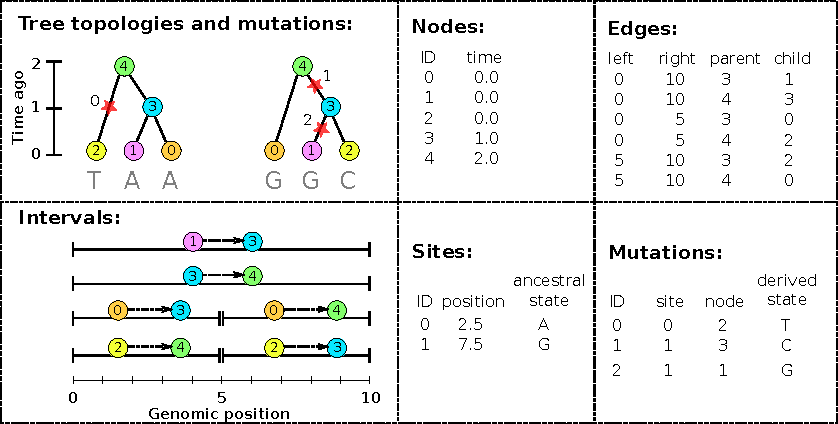
\includegraphics[width=\textwidth]{example_tree_sequence}
    \end{center}
    \caption{
        An example tree sequence with three samples over a chromosome of length 10.
        The left-hand panel shows the tree sequence pictorially in two different ways:
        (top) as a sequence of tree topologies 
        and (bottom) the spatial extent of the edges that define these topologies. 
        The right-hand panels show the specific encoding
        of this tree sequence in the four tables (nodes, edges, sites and mutations) 
        defined by \msprime.
        \plr{Whoops!  genotype of 1 in the second tree should be `G'!}
        \jk{Some minor alignment issues present here.}
        \plr{turns out this is no fun to edit in inkscape.  
            I can re-make to match the other figs
            but will leave alone for now: it's good!}
        \label{fig:example_tree_sequence}
    }
\end{figure}

The \emph{edges} define how nodes relate to each other over specific genomic intervals. 
Each edge records: 
% is a tuple $(\ell, r, p, c)$, where
the endpoints $[\ell, r)$ of the half-open genomic interval defining the
spatial extent of the edge; 
and the identities $p$ and $c$ of the parent and child nodes
of a single branch that occurs in all trees covering this interval.
The spatial extent of the edges defining the topology of Figure~\ref{fig:example_tree_sequence}
are shown in the bottom left panel. 
For example, the branch joining nodes 1 to 3 appears both trees,
and so is recorded as a single edge extending over the whole chromosome. 
It is this method of capturing the shared structure between adjacent trees that makes the
tree sequence encoding very compact and algorithmically efficient.

Recovering the sequence of trees from this information is straightforward:
each point along the genome that the tree topology changes
is accompanied by the end of some \emph{edges} and the beginning of others.
Since each \emph{edge} records the genomic interval 
over which a given node inherits from a particular ancestor,
to construct the tree at a certain point in the genome
we need only retrieve all edges overlapping that point
and construct the corresponding tree.
To modify the tree to reflect the genealogy at a nearby location,
we need only remove those edges whose intervals do not overlap that location,
and add those new edges whose intervals do.
Incidentally, this property that edges naturally encode \emph{differences}
between nearby trees (e.g., as ``subtree prune and regraft'' moves)
allows for efficient algorithms that take advantage
of the highly correlated nature of nearby trees~\citep{kelleher2016efficient}.

Given the topology defined by the nodes and edges, \emph{sites} and \emph{mutations}
encode the sequence information for each sample in an efficient way. Each site
is associated with a position on the genome and an ancestral state. For example,
in Figure~\ref{fig:example_tree_sequence} we have two sites, one at position
2 with ancestral state `A' and the other at position 7 with ancestral state `G'. If
no mutations occur, all samples inherit the ancestral state at a given site.
Each mutation occurs above a specific node at a given site, 
and results in a specific derived state. 
Thus, all samples below the mutation node in the tree will inherit this state 
(unless further mutations are encountered). 
Three mutations are shown in Figure~\ref{fig:example_tree_sequence}, 
illustrated by red hexagons. 
The first mutation occurs at site zero (in the left-hand tree), and is a simple
mutation resulting in node $2$ inheriting the state 'T'. 
The second site (in the right hand tree) has two mutations: 
one occurring over node $3$ changing the state to `C', 
and a back mutation over node $1$ changing the state to `G'.

This encoding of a sequence of trees and accompanying mutational information is
very concise. To illustrate this, we ran a simulation of $500,000$ samples of a
$200$ megabase human-like chromosome ($N_e=10^4$ and per-base mutation and
recombination rates of $10^{-8}$ per generation) using \msprime. This resulted
in about 1 million distinct marginal trees and $1.1$ million infinite-sites
mutations. The HDF5 file encoding the nodes, edges, sites and mutations (as
described above) for this simulation consumed 157MiB of storage space. Using
the \msprime\ Python API, the time required to load this file into memory was
around 1.5 seconds, and the time required to iterate over all 1 million trees
was 2.7 seconds. In contrast, recording the topological information in Newick
format would require around 20 TiB and storing the genotype information
in VCF would require about 1 TiB --
a compression factor of 144,000.
Working with either the Newick or VCF encoding
of this dataset would likely require several
days of CPU time simply to read the information info memory.


%%%%%%
\subsection*{Recording the pedigree in forwards time}

To record the genealogical history of a forwards in time simulation
we need to record two things for each new chromosome:
the birth time, and the endpoints and parental IDs of each distinctly inherited segment,
which are naturally stored as the \emph{nodes} and \emph{edges} of a tree sequence.
For concreteness, here we write out in pseudocode how to run a neutral Wright--Fisher simulation
(but with overlapping generations) that records genealogical history in this way.
The simulation will run for $T$ generations,
and has $N$ haploid individuals, each carrying a single chromosome of length L.
For simplicity we sample exactly one crossover per generation.
The probability of death per individual each generation is $\delta$.
We will use
$\randomuniform(A)$ to denote an element of the set $A$ chosen uniformly at random 
(and each such instance represents and independent draw).

We begin in~\algref{W1} by allocating our initial population $P$
(a vector of $N$ node IDs),
and creating $N$ nodes with birth time $T$ generations ago, recorded in the
vector $\tau$. The set $E$ is used to store the edges that we output during the
simulation, and $n$ is the number of nodes created so far (and so, the ID of
the next node we create). Steps~\algref{W2} and~\algref{W3} simply loop over
the generation clock $t$ and individual index $j$. In~\algref{W4} we check if
an individual $P_j$ has died in this generation. If it has, we replace it in
steps \algref{W5}--\algref{W7}; if not, we proceed immediately to the next
individual. When an individual in the population dies, we first allocate
a new node with ID $n$ in~\algref{W5} and record its birth time. Then,
in step~\algref{W6} we choose two indexes $a$ and $b$ uniformly (giving us
parental IDs $P_a$ and $P_b$) and choose a breakpoint $x$. We record the effects of this
event by storing two new edges: one recording that the parent of node $n$
from $0$ to $x$ is $P_a$, and another recording that the parent of $n$
from $x$ to $L$ is $P_b$. We then complete the replacement event by incrementing
$n$, ready to represent the next new node.

\begin{taocpalg}{W}{Forwards-time tree sequence}
{Simulates a randomly mating population $P$ of $N$ haploid individuals,
with a probability of death per generation $\delta$ and a chromosome of length
$L$ for $T$ generations. Events are recorded in a node table $\mathcal{N}$
and edge table $\mathcal{E}$. Simplify is run every $s$ generations.
}

\algstep{W1.}{Initialisation.}{
Set $\mathcal{N} \leftarrow \mbox{NodeTable}()$ and $\mathcal{E}
\leftarrow \mbox{EdgeTable}()$ and $t \leftarrow T$.
 For $0 \leq j < N$, set $P_j \leftarrow \mbox{add}(\mathcal{N}, T)$.
}

\algstep{W2.}{Generation loop.}{ If $t = 0$ terminate.
Set $P' \leftarrow P$ and then set $t \leftarrow t - 1$ and $j \leftarrow 0$.
}

\algstep{W3.}{Individual loop.}{ If $j = N$ set $P \leftarrow P'$ and go to \algref{W2}.
}

\algstep{W4.}{Mortality.}{ If $\randomuniform([0, 1)) \geq \delta$ go to \algref{W8}.
}

\algstep{W5.}{New node.}{Set $u \leftarrow \mbox{add}(\mathcal{N}, t)$ and $P'_j \leftarrow u$.
}

\algstep{W6.}{Choose parents.}{Set $a \leftarrow \randomuniform(\{0, \dots, N - 1\})$,
    $b \leftarrow \randomuniform(\{0, \dots, N - 1\})$ and $x \leftarrow \randomuniform([0, L))$.
}

\algstep{W7.}{Record edges}{
Call $\mbox{add}(\mathcal{E}, (0, x, P_a, u))$ and $\mbox{add}(\mathcal{E}, (x,
L, P_b, u))$.
}

\algstep{W8.}{Loop tail}{Set $j \leftarrow j + 1$ and go to \algref{W3}.
}

\algstep{W9.}{Simplify}{TODO}


\end{taocpalg}

This algorithm records only the topological information resulting from the
forwards in time Wright-Fisher process, but it is straightforward to add
mutational information. This can be done in two different ways.
We can record mutations that occur during the simulation quite simply.
For example, in Algorithm~\algref{W} we would generate mutations after
we have recorded the edges joining the new node $n$ to its parents
$P_a$ and $P_b$ in step \algref{W7}.
For example, if we assume that mutations occur according to the infinite sites model
at rate $\mu$ per generation per unit length then there are 
$\mbox{Poisson}\left(\mu (r - \ell)(\tau_p
- \tau_c)\right)$ mutations on each edge $(\ell, r, p, c)$. Each of these mutations
will occur on a distinct site $x$ drawn uniformly from $(\ell, r]$ and be associated with node $c$.
It is straightforward to record this information during the simulation, but it
is significantly simpler and more efficient to generate these mutations
after the simulation has completed. 
% In the case of infinite sites mutations
% there is no difference between generating these mutations during the forwards
% in time simulation and after it has completed. We are using precisely the same
% information.

\begin{figure}
    \begin{center}
        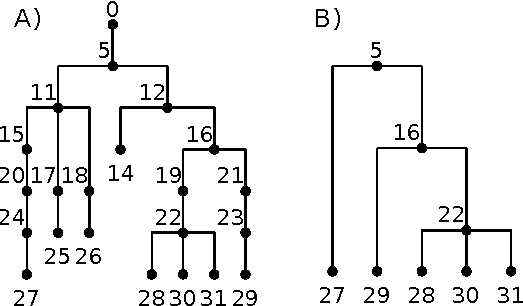
\includegraphics{wf-before-after}
    \end{center}
    \caption{An example of a marginal genealogy from a Wright-Fisher simulation
    with $N=5$. \textbf{(A)} the original tree including all
    intermediate nodes and dead-ends, and \textbf{(B)} the minimal tree
    relating all of the currently-alive individuals (27--31).
    \label{fig:wf-trees}
    }
\end{figure}

Besides the cost of transmitting genotypes,
generating mutations as a separate process after the topological simulation has completed 
avoids generating the many mutations that are lost in the population. 
Figure~\ref{fig:wf-trees} shows
an example of a marginal genealogy produced by a forwards-time Wright--Fisher
process like Algorithm~\algref{W}. 
On the left is the tree showing all the edges output by the simulation, 
while on the right
is the minimal tree representing the ancestry of the currently alive
population. Clearly there is a great deal of redundancy in the topological
information output by the simulation.

There are two sources of redundancy here. The first type of redundancy arises
from nodes in tree that have only one child. In Algorithm~\algref{W} we do
not attempt to track coalescence events but simply record all parent-child
relationships in the history of the population. As such, many of these edges
will record the simple passing of genealogical information from parent to child
and only some small subset will correspond to coalesences within the marginal
trees. The second source of redundancy in the output of Algorithm~\algref{W}
is due to the fact that lineages die out: a large number of
individuals in the simulation leave no descendants in the present day population. 
Node 26 in Figure~\ref{fig:wf-trees}a, for example, leaves no
ancestors in the current population, and so the entire path tracing back to
the root is redundant.

A minimal genealogy such as in Figure~\ref{fig:wf-trees}
has fewer edges on which to place mutations.
There are many more advantages to simplifying the genealogies to this point.
Computing this minimal representation of the
edges output by a forward-time simulation is an instance of a more
general problem that we cover in the next section.


%%%%%%
\subsection*{Tree sequence simplification}

Suppose that we are only interested in a subset of the nodes (our `samples')
of a tree sequence,
and so wish to reduce this input tree sequence
into the minimum representation of the topologies that include the specified
samples. The output tree sequence must have the following properties:
\begin{enumerate}
\item All marginal trees must match the subtree induced by the samples of the corresponding tree in the input tree sequence.
\item Within the marginal trees, all non-sample vertices must has at least
two children (i.e., unary tree vertices are removed), unless the vertex is a sample.
\item Any nodes and edges not ancestral to the sampled nodes are removed.
\item There are no adjacent redundant edges, i.e, pairs of edges $(\ell, x, p,
c)$ and $(x, r, p, c)$ which can be represented with a single edge
$(\ell, r, p, c)$.
\end{enumerate}


\begin{figure}
    \begin{center}
        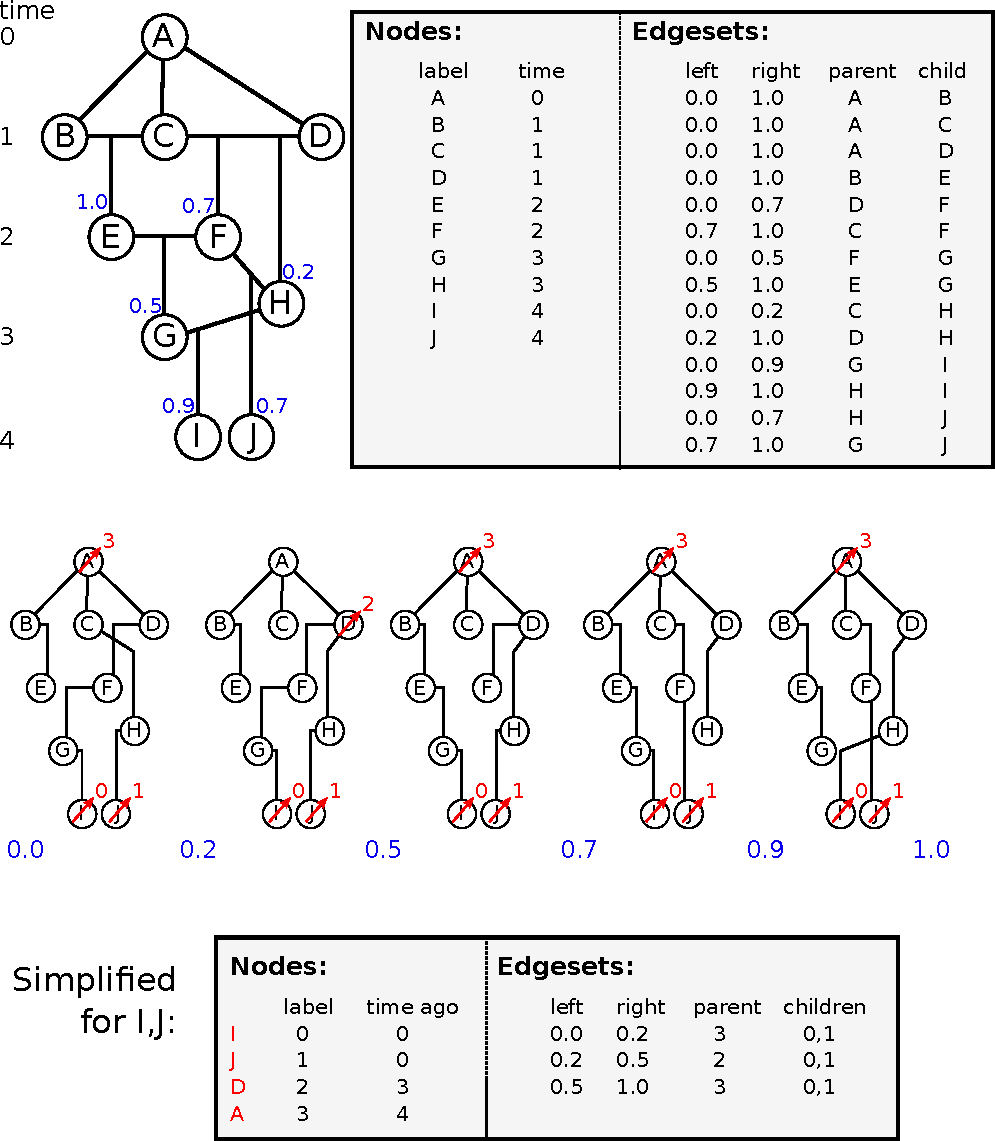
\includegraphics{method_diagram}
    \end{center}
    \caption{
        A simple example of the simplify method.
        \textbf{Top:} the diagram on the left relates ten haploid individuals to each other.
        It has 10 node records (one for each individual)
        and 14 edge records (one for each distinctly inherited segment).
        Blue numbers denote crossing over locations in each meiosis --
        for instance, $C$ and $D$ were parents to $F$,
        who inherited the left 70\% of the chromosome from $D$ and the remainder from $C$.
        The individuals $B$, $C$, and $D$ inherit clonally from $A$.
        \textbf{Center:} the five distinct trees relating all individuals to each other
        found across the chromosome (blue numbers denote locations on the chromosome).
        Labels after simplification are shown in red.
        \textbf{Bottom:} tables recording the tree sequence after simplification
        with nodes $I$ and $J$ as samples.
        The mapping from labels in the forwards time simulation to nodes in the tree sequence
        is shown in red.
        % which allows additional records to be added as the simulation progresses.
        \label{fig:method_diagram}
    }
\end{figure}

The tree sequences produced by forwards simulations 
record all of history for everyone alive at any time through the simulation.
This is much more than we need to reconstruct the genealogies and sequences
of the current population.
Simplification is essential to reduce this 
to a manageable quantity that still contains all
the information that we are interested in. 
Simplification is also useful if we have a
large tree sequence representing a large dataset and we wish to extract the
information relevant to a subset of the samples.

The approach that we take is based on Hudson's algorithm for simulating
the coalescent with recombination~\citep{hudson1983properties,kelleher2016efficient};
the implementaiton of simplify parallels the implementation of Hudson's algorithm in \msprime.
Conceptually, this works by 
(a) beginning by painting the chromosome each sample a distinct color;
(b) moving back through history, 
copying the colors of each chromosome to the portions of its' parental chromosomes
from which it was inherited;
(c) each time we would paint two colors in the same spot (a coalescence),
record that information as an edge and instead paint a brand-new color; 
and
(d) once all colors have coalesced on a given segment,
stop propagating it.
This ``paint pot'' description misses some details --
for instance, we must ensure that all coalescing segments in a given individual
are assigned the \emph{same} new color --
but is reasonably close.
The process is depicted in Figures~\ref{fig:method_diagram} and \ref{fig:simplify_state}.

\begin{figure}
    \begin{center}
        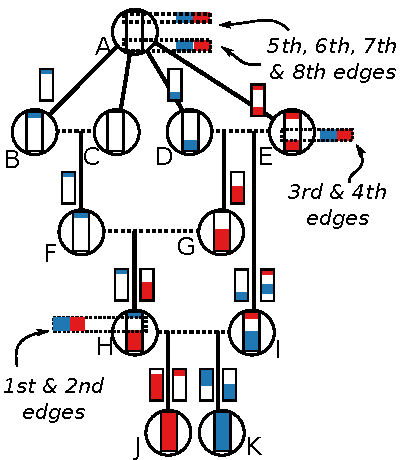
\includegraphics{simplify-state-diagram}
    \end{center}
    \caption{
        A depiction of the state of the simplification algorithm
        at each point in time,
        in the example of Figure~\ref{fig:method_diagram}.
        \label{fig:simplify_state}
    }
\end{figure}

More concretely,
the algorithm works by moving back through time,
processing each parent in the input tree sequence in chronological order.
The main state of the algorithm at each point in time is a set of ancestral lineages,
and each lineage is a collection of ancestral segments.
An ancestral segment $(\ell, r, u)$ is found in a lineage
if the output node $u$ inherits the genomic interval $[\ell, r)$ from that lineage.
% These segments are stored in a collection of linked lists,
% one list of segments for each ancestral lineage present at that time.
(These lineages are the ``colors'' above.)
We also maintain a map $A$ such that $A_j$ is segment chain for node $j$ in
the input tree sequence.
Crucially, the time required to run the algorithm is linear in the number of edges of the input tree sequence.

\subsection*{Forward simulation and sequential simplification}

At any point in a simulation scheme like Algorithm~\algref{W}, genealogical history is recorded
in a tree sequence. This has two additional advantages. First, simplification
can be run periodically through the simulation, taking the set of samples to be
the entire currently alive population. This is important as it keeps memory
usage from growing linearly (and quickly) with time. Second, the simulation can
be \emph{begun} with a tree sequence produced by some other method -- for
instance, by a coalescent simulation with \msprime. 
This process of forward simulation coupled with sequential simplification is our
method

\jda{I didn't write down the full thing, but mightn't things be clearer if we
	have a statement of the combined method?}
\begin{taocpalg}{F}{Forwards-time simplifed tree sequence}{
Simulates a population starting with $N$ diploid individuals on a chromosome of length $L$ for $T$
generations.
}

\algstep{F0.}{Initialize nodes.}{
Generate initial haploid nodes $\mathcal N$:
1.) using coalsecent simulation with \msprime{} for $2N$ initial haploid samples $S$ on
a chromosome of length $L$ and taking $\mathcal N = \{\texttt{id}(u) : u \in S \}$; or
2.) simply defining $\mathcal N = \{1\dots 2N\}$ as the node ids.
Define a mapping from  $\mathcal M: \{1\dots 2N\} \to \mathcal N$. In the second
case $\mathcal M$ is the identity.
}

\algstep{F1.}{Initialize edges.}{
Define the initial edges $E_0$: 1) either from the coalescent simulation's final
state, or 2) as \dots
}

\algstep{F2.}{Record trees till time $T - \Delta$.}{ 
Simulate, using Algorithm~\algref{W} or another algorithm, $2N$ haploid
individuals using $\mathcal M$ to renumber the nodes, producing nodes $n$ and
edgesets $E$.
}

\algstep{F3.}{Simplification over $\Delta$.}{
Select final samples $S'$ and using the simplification Algorithm~\algref{S},
simplify $n$ and $E$ to produce a simplified tree sequence.
}

\algstep{F4.}{Continue?}{
	Stop if $T - \delta  = 0$, else continue.
}
\end{taocpalg}


%%%%%%%%%%%%
\subsubsection*{Estimates of run-time complexity}

\jda{I'd like to outline what we're doing here with reference to alg F}
Consider a simulation of a Wright-Fisher population of $2N$ haploid individuals 
using Algorithm~\algref{W}
for $T$ generations,
with the probability of death, $\delta$, set to 1 for simplicity.
Since there is exactly one crossing over every generation,
this produces tables of 
$2NT$ nodes and
$4NT$ edges.
Suppose that $T$ is large enough that all samples coalesce within the simulation with high probability,
so that $T \sim 20N$, say.
After simplification, we are left with the tree sequence describing the history
of only the current generation of $2N$ individuals.
This tree sequence has $4N-2$ edges to describe the leftmost tree;
and each time the marginal tree changes along the sequence,
three edges end and three new edges begin (except for changes affecting the root; see \citet{kelleher2016efficient}).
Coalescent theory tells us that 
the expected total length of edges in a marginal tree is approximately $4N\log(2N)$,
which is also equal to the mean number of ancestral recombination events that occur on a branch of the marginal tree,
since we have taken one crossover per generation.
Not all such recombinations actually change the tree topology,
and three times this gives us an upper bound on the expected number of edges.
Similarly, not every new edge derives from a never-before-seen node,
but the number of nodes is at most equal to the number of edges plus the sample size.
With $T=20N$, this reduces the initial storage of $160 N^2$ items to $8N(4\log(2N) + 3)$;
at $N=10^4$, a factor of 4,700.

To get an idea of how required space depends on the length of time,
suppose instead that we have run a simulation of $2N$ individuals for $T$ generations,
begun with no prior history.
This produces $4NT$ edges; how many are required after simplification?
As above, the expected number of edges is bounded by $2N-2$ plus four times the mean marginal tree length.
Roughly, the length of time for which a marginal tree has k tips is 
$2N/k(k-1) = 2N(1/(k-1) - 1/k)$,
and so the time to go from N to n tips is $2N(1/(n-1) - 1/(N-1))$.
This implies that after running for time $T$ we expect to 
have around $n(T)$ roots, where $n(T) \approx 1 + 2N/(T+2)$.
The total tree length over this time is 
$2 N \sum_{k=n(T)+1}^{N-1} 1/k$, which 
% is approximately
% \begin{align*}
%     2 N \log\left( \frac{N}{1 + 2 N/(T+2)} \right) .
% \end{align*}
leads to an upper bound on the number of edges of
\begin{align*}
    2 N \left( 1 + 4 \log\left( \frac{NT}{T + 2 N} \right)\right) .
\end{align*}
This holds up quite well in practice --
the number of edges actually required for 50 independent Wright--Fisher simulations,
as a function of time (obtained by running simplify every generation)
is shown in \ref{fig:num_edges}, compared to this prediction.

\begin{figure}
    \begin{center}
        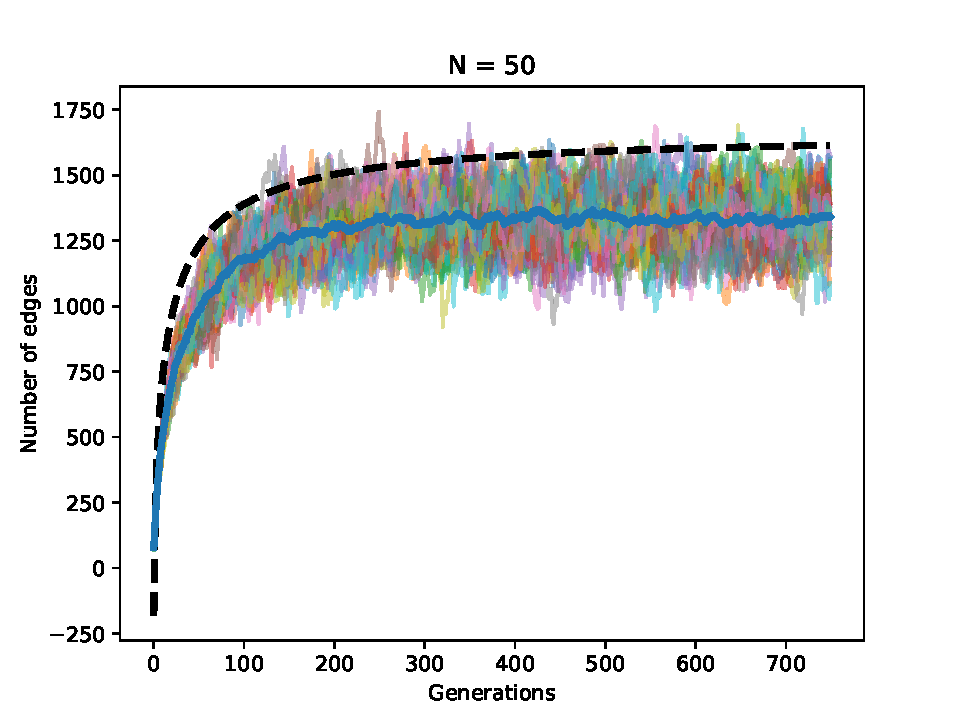
\includegraphics{sims/num_edges_50}
    \end{center}
    \caption{
        Number of edges in the simplified tree sequence
        for 50 Wright-Fisher simulations begun with no prior history
        as a function of number of generations.
        Each line is one simulation, the black line gives the average,
        and the dotted line is the upper bound of the text.
        \label{fig:num_edges}
    }
\end{figure}
 

If we were to add mutations in forwards time 
under the infinite-sites model with total mutation rate per generation $\mu$,
there would also be around $\mu 2NT$ mutations (and the same number of sites).
Since mutations fall as recombinations do on the marginal trees,
adding them after simplification results in only around $\mu 4 N \log(2N)$ mutations.
This furthermore avoids the computational burden of propagating mutations forwards through the generations.

Our method stores genealogies, and so records substantially more information 
than would a method only recording genotypes.
However, since the simplification algorithm requires some computational effort,
it is still informative to compare computational complexity of the algorithm
to one that propagates neutral genotypes.
A typical individual will differ at $2 N \mu$ sites from the population's consensus sequence,
so propagating these to offspring by simple copying will take $4 N^2 \mu$ operations per generation.
On the other hand, we must store $13N$ quantities per generation (two edges and one node per individual).
The simplification algorithm is linear in the number of edges of the input tree sequence,
and so multiplies this by a constant factor.
Concretely, propagating neutral genotypes for $T$ generations has time complexity $O(\mu T N^2)$,
while our implementation is only $O(T N \log(2N))$.


\subsection*{Simulation benchmarks}

Comparison of simulation with/without msprime, using \simupop{}
or maybe just a simple haploid simulation with 1000 QTL and stabilizing selection on a trait (say).

Maybe an estimate of how long \emph{just} the ARG recording and simplification takes,
so that then we can say how fast the simulator would have to be to do $10^6$ whole chromosomes for $10^7$ generations
in a day.


%%%%%%%%%%%%%%%%%%%%%%
\section*{Discussion}

In this paper, we have shown that storing pedigrees
and associated recombination events
in a forwards-time simulation
not only results in having available a great deal more information about the simulation,
but also can speed up the simulation by orders of magnitude.
To make this feasible, 
we have described how to efficiently store this information in tables,
and have described a fundamental algorithm for simplificication of tree sequences.
Conceptually, recording of genealogical and recombination events
can happen independently of the details of simulation;
for this reason, we provide a well-defined and well-tested API in C and in python
for use in other code bases.

The tree sequences produced by default by this method
are very compact, storing genotype \emph{and} genealogical information
in a small fraction of the space taken by a compressed VCF file.
The format is also highly efficient to process,
leading to advantages for downstream analysis as well.
This is because many algorithms to compute statistics of interest for population genetics
are naturally expressed in terms of tree topologies,
and so can be quickly computed from the trees underlying the tree sequence format. 
For example, pairwise nucleotide diversity $\pi$, is the average density of
differences between sequences in the sample. 
To compute this directly from sequence data at $m$ sites in $n$ samples
requires computing allele frequencies, taking $O(nm)$ operations.
By using the locations of the mutations on the marginal trees,
and the fact that these are correlated, 
dynamic programming algorithms similar to those in~\citep{kelleher2016efficient}
can do this in roughly $O(n + m \log n)$ operations.
The \msprime\ API provides a method to compute $\pi$ among arbitrary subsets of the
samples in a tree sequence, which took about 1.2 seconds
applied to the example tree sequence above with 1.1 million mutations 
in 200 megabases for 500,000 samples.

Another attractive feature of this set of tools
is that it makes it easy to incorporate \emph{prior history},
simply by seeding the simulation with a (relatively inexpensive) coalescent simulation.
This allows for incorporation of deep-time history beyond the reach of individual-based simulations. 
Since geographic structure from times longer ago than the mixing
time of migration across the range has limited effect on modern genealogies
\citep{wilkins2004separation} (other than possibly changing effective population
size \citet{barton2002neutral,cox2002stepping}), this may not negatively affect realism.


A final note:
in preparing this manuscript, 
we debated a number of possible terms for the embellished pedigree,
i.e., the ``pedigree with ancestral recombination information''.
Current etymologica consensus \citep{liberman2014little} has
``pedigree'' derived from the french ``pied de grue'' for the foot of a crane
(whose branching pattern resembes the bifurcation of a single parent-offspring relationship).
An analogous term for the embellished pedigree might be \emph{nedigree},
from ``nid de grue'',
as the nest of a crane is a large jumble of (forking) branches.
We thought it unwise to use this term throughout the manuscript,
but perhaps it will prove useful elsewhere.


%%%%%%%%%%%%%%%%%%%%%%
\section*{Methods}

\plr{some of this can move back to an appendix, but since they want methods at the end,
it's the sort of thing they want here.}

%%%%%%%%%%%%%%
\subsection*{Simuation methods}

Jaime and Kevin to describe simulation methods here (separately).

%%%%%%
\subsection*{Overview of the API}

The \msprime{} Python API provides a powerful platform for working with tree topology and mutation data. 
The new portions of \msprime{} that we cover here
are dedicated to tree sequence input and output using simple tables of data,
so we refer to this as the `Tables API'.
The four key tables: nodes, edges, sites and mutations, are described above.

The Tables API is primarily designed to facilitate efficient interchange of
data between programs or between different modules of the same program.
\jda{should capitalize Tables, or not, as above}
Following the current best-practises [citations: apache arrow, etc] data is stored
in a columnar format.
The principal advantage of this for our purposes is that it allows for very efficient
interchange of large amounts of numerical data. In principle, this enables
zero-copy semantics, where a data consumer can read the information directly
from the memory of a producer without incurring the overhead of a copy
[citation?] Our implementation uses the numpy C API [citation] to efficiently copy
data from Python into the low-level C library used to manipulate
tree sequences.
Thus, by using a simple numerical
encoding of tree topologies and contiguous arrays of data to store this
encoding, we can achieve data transfer rates that would be impossible under
any text-based approach while retaining excellent portability.


The \msprime{} tables API is independent of the details of a particular simulation engine.  In other words, one simply
needs to fill the relevant columns and send them to \msprime{} at regular intervals for simplification.  For example,
using the \fwdpp{} C++ API \cite{Thornton2014-hx}, we fill arrays of simple structures representing the node and edge data.
Doing so requires no modification of the \fwdpp{} code base.  Rather, we simply need to book-keep the parent/offspring
labels and perform simple processing of the recombination breakpoints from each mating event.  Using \texttt{pybind11}
(\url{https://github.com/pybind/pybind11/}),
the node/edge arrays on
the C++ side are made visible, without copy, to Python as a multi-column numpy array. This array is in turn processed by
the \msprime{} tables API.  In order to create a standalone user interface, our implementation uses \texttt{pybind11} to
create a Python package extending \texttt{fwdpy11} (\url{https://github.com/molpopgen/fwdpy11}), which is a Python
package based on \fwdpp{}.  (A neat aside, that we may wish to skip here, is that it may be possible to use the tables
API from a command-line C/C++ application via an embedded Python interpreter.)
\plr{@molpopgen: note on how this works with fwdpp?}
\krt{@plr: done, but perhaps too verbose?}

The tables API provides basic input and output operations via the numpy
array interface, which provides a great deal of flexibility as well
as efficiency, and makes it straightforward to transfer data from sources
such as HDF5 [citation], Dask, or Zarr. 
(For small scale data and debugging purposes, a simple text format is also supported.)
Along with these operations we also provide a function to sort a set of tables
to ensure that the records are in the form required to input
into an \msprime{} tree sequence object. (Simplification may also be required.)

\plr{Maybe we don't need this paragraph? Already said it, more or less, above, esp if we insert something about how fwdpp works.}
\jda{agree re the next two lines. propose moving the other above}
This interchange API is very efficient. [Describe a quick example where we generate
a many-gigabyte tree sequence using fwdpp, and the time required
to copy the node and edge data into the tables].

%%%%%%%%%%%%%%
\subsection*{The table format}

Given a set of node and edge tables as described above,
there are a small set of requirements that ensure the tables
describe a valid tree sequence.
(There are essentially no such requirements on the site and mutation tables.)
These are:
\begin{enumerate}
    \item Offspring must be born after their parents (and hence, no loops).
    \item The set of intervals on which each individual is a child must be disjoint.
\end{enumerate}
A pair of node and edge tables that satisfy these two requirements
is guarenteed to uniquely describe at each point on the genome
a collection of directed, acyclic graphs -- in other words, a forest of trees.
For some applications it is necessary to check that at every point
there is only a \emph{single} tree.  
Checking this is more difficult, but is implemented in \msprime{}'s API.
\jda{TODO add function name}

For efficiency, \msprime{} makes several other sortedness requirements on the tables,
that are not necessarily satisfied by tables emitted by a forwards-time simulation.
\msprime{}'s API includes tools to rectify this by first sorting (using \texttt{sort\_tables})
and then using \texttt{simplify}, which works on sorted tables
and is guarenteed to produce a valid, \msprime{}-ready tree sequence.

Note that since each node time is equal to the amount of time since the \emph{birth} of the
corresponding parent, time is measured in clock time, not in meioses.
\jda{is this the right place? I'd put it in discussion of Figure~\ref{fig:example_tree_sequence}}


%%%%%%%%%%%%%%
\subsection*{Simplification}

Here we describe the simplification algorithm.
The flow is close to our implementation,
but the description below uses set operations,
while in the implementation,
all ancestors are maintained as linked lists of segments
ordered by left endpoint.

\begin{taocpalg}{S}{Simplify a tree sequence}
{Simplifies the input tree sequence:
    input consists of 
    a list of sample IDs, $S$, of length $n$,
    a list of edges, $\mathcal{E_I}$,
    and a list of nodes $\mathcal{N_I}$.
    The genome length is $L$.
    The output will be stored in a list of edges $\mathcal{E_O}$ 
    and nodes $\mathcal{N}_O$.
    This also maintains the list $N$ that gives the mapping 
    from $\mathcal{N_I}$ to $\mathcal{N_O}$,
    so that if $M[p] = u$ then the $p^\text{th}$ ancestor in $N_I$
    is the same as the $u^\text{th}$ ancestor in $N_0$.
    The internal state is $\mathcal{A}$, the list of ancestors
    (which are collections of ancestral segments).
}

\algstep{S0.}{Initialize.}{
    Set $\mathcal{A}[j] \leftarrow (0, L, j)$ 
    and $\mathcal{N}_O[j] \leftarrow \mathcal{N}_I[S[j]]$ for $0 \le j < N$.
    Set $Q \leftarrow \emptyset$,
    and $M[p] \leftarrow -1$ for $0 \le p < \text{length}(N_I)$.
}

\algstep{S1.}{Input parent loop.}{Loop over parents, chronologically.
}

\algstep{S2.}{Remove ancestry.}{Call Algorithm \algref{R} 
    on each edge corresponding to the current parent.
}

\algstep{S3.}{Merge ancestors.}{Merge the resulting segments into a new ancestor for this parent.
}

\end{taocpalg}

The first step is, for each edge $(\ell, r, p, c)$,
simply to replace any ancestry segment $[a, b)$ held by ancestor $c$
with $[a,b) \setdiff [\ell, r)$ 
(deleting the segment or splitting in two if necessary),
and adding the removed segment $[a,b) \cap [\ell, r)$ to the merge queue $Q$:
\begin{taocpalg}{R}{Remove ancestry}
    {Given an edge $(\ell, r, p, c)$,
    and a list $\mathcal{A}[c]$ of the $m$ ancestral segments corresponding to $c$,
    remove segments overlapping $[\ell, r)$ from $\mathcal{A}[c]$,
    and add those overlapping segments to $Q$.
    }

    \algstep{R1.}{Segment loop.}{Loop over ancestral segments in $\mathcal{A}[c]$:
    if $j=m$, terminate; else let $(a, b, u) = \mathcal{A}[c][j]$.
    }

    \algstep{R2.}{Add to merge queue.}{If $[a,b) \cap [\ell,r) \neq \emptyset$,
    append $(\max(a,\ell), \min(b,r), u)$ to $Q$.
    }

    \algstep{R3.}{Remove ancestry.}{If $[a,b) \cap [\ell,r) != \emptyset$,
    delete $\mathcal{A}[c][j]$ and insert in its place
    $(\min(a,\ell), \max(a,\ell), u)$ (if $a<\ell$) 
    and/or $(\min(b,r), \max(b,r), u)$ (if $r<b$).
    }

\end{taocpalg}

Next we must merge these ancestry segments,
creating the new ancestor $p$,
outputting edges and a node if coalescence has occurred.
\begin{taocpalg}{M}{Merge ancestors}
    {Merge a collection of segments and create a new ancestor.
    This operates on the merge queue $Q$ above,
    which is a list of ancestral segments,
    and creates the new ancestor $\mathcal{A}[p]$.}

    \algstep{M1.}{Segment loop.}{While $\mathrm{length}(Q)>0$:}

    \algstep{M2.}{Find next segment overlap boundaries}{
    Let $\ell \leftarrow \min\{x.\ell : x \in Q\}$
    and $H \leftarrow \{x \in Q : x.\ell = \ell\}$.
    Also let $\ell_+ \leftarrow \min\{x.\ell : x \in Q \setdiff H\}$
    and $r = \min(\ell_+, \min\{x.r : x \in H\})$.
    }

    \algstep{M3.}{Copy single segment.}{If $\mathrm{length}(H) == 1$,
    set $\alpha \leftarrow (\ell, r, H[0].n)$.
    If also $p \in S$, then append $(\alpha.\ell, \alpha.r, N[p], \alpha.c)$ to $\mathcal{E}_O$
    and then set $\alpha.c \leftarrow M[p]$.
    Go to \algref{M7}.
    }

    \algstep{M4.}{Coalescence head.}{If $(h \leftarrow \mathrm{length}(H)) > 1$,
    if $M[p] == -1$ set $M[p] \leftarrow \text{length}(N_O)$
    and append $N_I[p]$ to $N_O$.
    Set $\alpha \leftarrow (\ell, r, M[p])$.
    }

    \algstep{M6.}{Record edges.}{
    For each $x \in H$, append $(\ell, r, M[p], x.n)$ to $\mathcal{E}_O$.
    }

    \algstep{M7.}{Update $Q$.}{
    Set $Q \leftarrow Q \setdiff \{x \in Q : x.r == r\}$
    and then set $x.\ell = \ell$ for all remaining $x \in Q$.
    }

    \algstep{M8.}{Add segment to ancestor.}{
    Append $\alpha$ to $\mathcal{A}[p]$ and return to \algref{M1}.
    }

\end{taocpalg}



%%%%%%%%%%%%%%%%%%%%%%
\section*{Acknowledgements}
Thanks to Brad Shaffer and Evan McCartney-Melstad for useful discussions.
Funding for this project cam from XXX


\bibliography{references}

\appendix


\end{document}
